\section{Durchführung der Aufgabe}

In diesem Kapitel beschreiben wir konkret, wie die Arbeit während meines Praxissemesters sich entwickelte. Die ersten zwei Wochen dienten als Einarbeitung und Einstieg. Nach dieser Phasen bekam ich langsam und unter Betreuung mehr Verantwortlichkeit und mehr Freiheit, um die Arbeit durchzuführen. In der folgenden Tabellen wird der Ablauf systematisch und ohne Einzelheit beschrieben. In dem zweiten Teil dieses Kapitels geben wir eine ausführliche Beschreibung eines Projekts.

Jedes Projekt besitzt innerhalb von Wallsec einen festgelegten Aufbau. Dieser kann in den folgenden Punkten zusammengefasst werden:

\begin{enumerate} \label{Projektablauf}
    \item \textit{Kick-off Meeting} mit den Kunden, um grundsätzliche Information über die Anwendung zu bekommen
    \item Definition der Umfang des Tests, wie Anmeldedaten, Rolle der zu getestete Nutzer, \glsplural{Tennant} und Einschränkungen
    \item Durchführung von Tests nach einem vorgegebenen Checklist
    \item Dokumentation der durchgeführten Testen, dessen gefundene \glsplural{Schwachstelle} und Vorschläge zur Härtung der Anwendung
    \item Abschlussmeeting mit dem Kunden, um die \glsplural{Schwachstelle} und deren Ausnutzung zu präsentieren und zu demonstrieren
\end{enumerate} 

\section{Wöchentliche Zusammenfassung meines Praxissemesters}

\begin{table}[H]
    \setstretch{1.0}
    \begin{tabularx}{\textwidth}{|c|X|}
    \toprule
    \multicolumn{2}{c}{\textbf{Auflistung der Aufgabe}} \\
    \midrule
    \multicolumn{1}{c}{\textbf{Woche}} & \multicolumn{1}{c}{\textbf{Aufgabeschreibung}} \\
    \hline
    1 - 2    & Einarbeitung:
                \begin{itemize}
                    \item Installation von einer virtuellen Maschine für die Testumgebungen
                    \item Einführung in der Arbeitsablauf der Firma
                    \item Einführung, Installation und Einstellungen von \gls{burp}
                    \item Einführung in einem laufenden Projekt, um über das Ablauf- und Dokumentationsverfahren zu lernen
                    \item Durchführung und Wiederholungen von einigen Tests, um mich an den gegebenen Tools zu gewöhnen
                    \item Teilnahmen an einer Abschlussmeeting des laufenden Projekts, um das Verfahren und den Ablauf des Kundenkontakt zu erkennen und später zu wiederholen
                \end{itemize} \\
        \hline

    3 - 4       &  Start, Durchführung und Abschluss eines neuen Pentesting-Projekts an einem Versicherungsanwendung mit dem obigen beschriebenen Schritte (\ref{Projektablauf})  \\ 
    
    \hline

    5 - 6       & Weiterarbeitung an der Installation, an der Einstellungen und an der Nutzung der Tools \gls{TheHive} und \gls{Cortex}. Bereitstellung von Skripts zum Herunterladen von statistische Daten der Anwendungen und zur Automatisierung deren Nutzung.  \\ 

    \hline

    7 - 8      &  Start, Durchführung und Abschluss eines neuen Pentesting-Projekts an einem Marketing-Webanwendung mit dem obigen beschriebenen Schritte (\ref{Projektablauf}) \\

    \hline

    9 - 10      &  Start, Durchführung und Abschluss eines neuen Pentesting-Projekts an Netzwerk-Umgebungen mit dem obigen beschriebenen Schritte (\ref{Projektablauf}). Die durchgeführten Tests konzentrieren sich auf die Sicherheit einer Netzwerk in einer Cloud-Umgebung. Für dieses Projekt spielen die Tools \gls{nmap} und \gls{scout} eine wichtige Rolle, da das Ziel war, Hosts, Dienste und dessen Einstellungen und \gls{Schwachstelle} zu erkennen \\

    \hline

    13 - 14      &  xxxxxx \\

    \hline

    15 - 16      &  xxxxxx \\


    \hline

    17 - 18      &  xxxxxx \\

    \hline

    19 - 20      &  xxxxxx \\


       \bottomrule
    \end{tabularx}
\end{table}

\section{Ausführliche Beschreibung eines Penetration Testing innerhalb des Praxissemesters}

Bevor der Durchführung jedes Tests ist Wallsec und ihre Mitarbeiter dazu verpflichtet, eine Vertraulichkeitserklärung zu unterschreiben. Keine Information weder über die Firma noch über die verwendeten Methode dürfen aus irgendwelcher Form veröffentlicht werden. Aus diesem Grund werden die hier demonstrierten Methode und Tests in der Test- und Lernumgebung \glsfirst{dvwa} gezeigt. In den realen Tests verwenden wir ähnliche Methode, manchmal mit mehr oder weniger Details, um die Sicherheit der Anwendungen zu überprüfen. 

Obwohl jede Webanwendungen ihre eigene Eingenschaften haben, besitzen fast alle eine ähnliche Struktur und Aufbau. Beim jeden Test fangen wir damit an, diese gemeinsame Struktur zu erkennen, indem wir nach öffentlichen Informationen suchen. Viele kritische Informationen, wie Username, Passwörter, Versionen, Systemen verbundenen IP-Adressen, lassen sich sehr leicht nach einer Online-Suche finden. Auch mit eingebauten Tools eines Betriebssystems können wir auf solche Informationen zugreifen. Dieses Verfahren nennen wir Banner Grabbing. Das folgende Bild zeigt ein Beispiel von einer einfachen Durchführung von Banner Grabbing:

\begin{figure}[h]
    \centering
    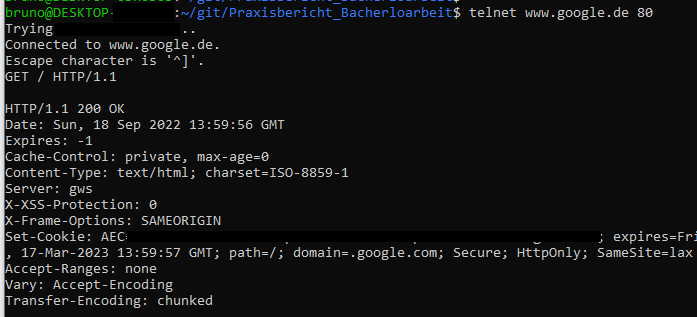
\includegraphics[width=0.5\textwidth]{/home/bruno/git/Praxisbericht_Bacherloarbeit/Praxissemester/assets/banner_grabbing.png}
    \caption{Banner Grapping mithilfe von dem Tool telnet}
    \centering
\end{figure}

\subsection{Suche nach versteckten Dateien und oder Verzeichnisse}

Eine Webanwendung ist eine Gruppierung von verschiedene Verzeichnisse. Jedes Verzeichnis soll den Nutzer eine Information oder Interaktion anbieten. Manche sind aber nicht für Nutzer gedacht und dient hauptsächlich dazu, Einstellungen zu verwalten. Da solche Verzeichnisse nicht dazu konzipiert, direkt aufrufbar zu sein, benutzen wir Testers andere Methode, um zu finden, was die Entwickler im Hintergrund beibehalten wollte. Es gibt verschiedene Tools, die mithilfe von sogenannten \textit{wordlists}, viele Anfrage an eine Anwendung schickt, um herauszufinden, was nicht direkt von dem Browser aufrufbar ist. Solche \textit{wordlists} sind Textdateien, die häufige verwendete Wörter beinhalten, die für Webanwendungen, für Nutzername oder für Passwörter verwendet werden. Da viele Webanwendungen ähnliche Strukturen haben, ist auch meistens erwartet, dass gewöhnliche Wörter auch zu finden sind. Das nächste Beispiel zeigt uns, dieses Entdeckungsverfahren auf unserem Ziel, \gls{dvwa} Tool. Hier benutzen wir das Tool \gls{dirb}, um herauszufinden, welche Verzeichnisse in dieser Anwendung existieren. Dieses und andere Tool arbeiten mit der Brute-Force Methode. In diesem Fall werden verschiedene Anfrage geschickt, jede mit einem verschiedenen Wort, um zu sehen, welche positive Antworten liefern. Das folgende Bild zeigt die Durchführung und das Ergebnis des Scanverfahren mithilfe des Tools \gls{dirb}:

\begin{figure}[h]
    \centering
    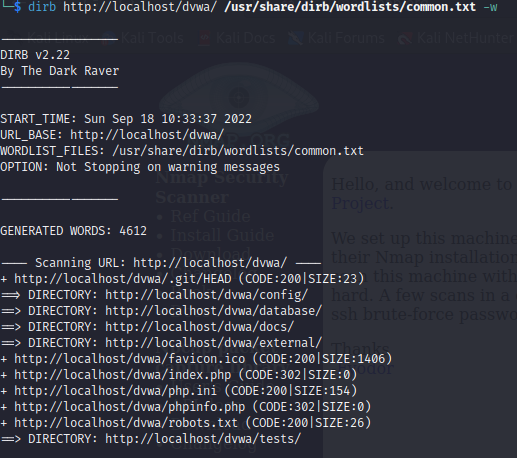
\includegraphics[width=0.5\textwidth]{/home/bruno/git/Praxisbericht_Bacherloarbeit/Praxissemester/assets/dirb.png}
    \caption{Brute force Scan für Verzeichnisentdeckung}
    \centering
\end{figure}

Der nächste Schritte wäre eine manuelle Beobachtung der entdeckten Material, um zu finden, ob irgendwelche sensitiven Information ausgelieferte wurde. Falls ja, wurden wir dann versuchen diese \gls{Schwachstelle}, zu erkennen und auszunutzen.

\subsection{Suche nach laufenden Dienste}

Ein Netzwerk-Scan ist auch eine häufige verwendete Methode, um zu finden, auf welche Dienste oder Anwendungen unser Ziel gebaut ist. Dieses Scan schickt an dem Ziel verschiedene Anfrage, damit wir das Reaktion des Zielsystems beobachten können. Während bei dem ersten Scan wir uns auf der Webanwendung fokussierten, hier bearbeiten wir eine Ebene, die nicht für normale Nutzung gezielt ist. Unser Fokus hier liegt auf dem Server, wo die Anwendung läuft. Dafür testen wir die sogenannte \gls{port}. Aus diesem Scan lassen sich meistens viele nützliche Informationen herausfinden, wie Betriebssystems, wo die Webanwendung läuft, Name und Versionen der existierenden Dienste. Mit dieser Information ist es möglich dann zielgerichtete Angriffe vorzubereiten, um \glsplural{Schwachstelle} auszunutzen.

Das nächste Bild zeigt das Ergebnis der Durchführung von \gls{nmap} gegen das Testziel \textit{scanme.nmap.org}:

\begin{figure}[h]
    \centering
    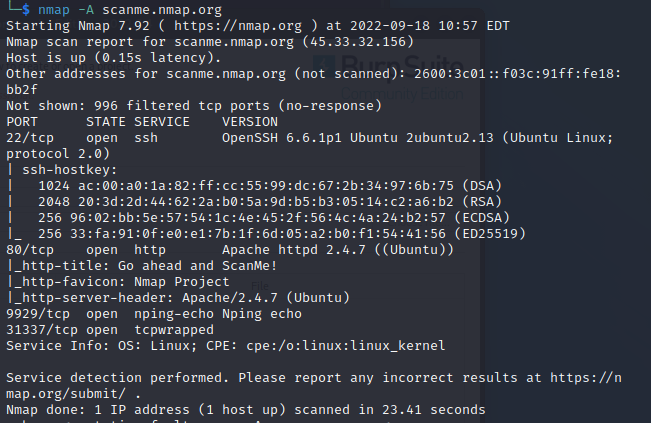
\includegraphics[width=0.5\textwidth]{/home/bruno/git/Praxisbericht_Bacherloarbeit/Praxissemester/assets/nmap.png}
    \caption{Brute force Scan für Verzeichnisentdeckung}
    \centering
\end{figure}

Aus diesem Scan erfahren wir welche Betriebssystem und welche Version der Webanwendung benutzt werden. Auch wenn solche Versionen gegen Angriffe geschützt sind, ist es unsere Aufgabe dem Kunde zu informieren, dass sensitive Informationen für alle sichtbar sind. Eine böse absichtliche Nutzer könnte diese Information nutzen, um eine \glsplural{Schwachstelle} für diese Anwendungen zu erfinden und dann auszunutzen.

\subsection{Typische Webanwendungen Tests}

Nachdem die vorherigen Scans durchgeführt wurde und öffentliche und Serverseite Informationen gesammelt wurden, fangen wir damit an, die Webanwendung direkt zu testen. In diesem Fall ist es unser Ziel zu wissen, welche versteckte Daten oder unerlaubte Aktionen ein Angreifer durchführen kann, um die \gls{CIA} der Anwendung zu verletzen. Für die folgenden Tests benutzen wir hauptsächlich das Tool \gls{burp}.

